\chapter{Introduction} % Write in your own chapter title
\label{Chapter1}
\lhead{} % Write in your own chapter title to set the page header

\section{Motivation}
The objective of our project is to explore the potential of deep neural networks in areas of information processing and medical sciences. We have observed its potential in Computer vision and acoustics, and we believe that these avenues have a lot of potential for improvement as well. Currently, these areas are saturated with hand-crafted algorithms which are closed-form mathematical solutions to messy natural phenomenon like communication-channels or clinical data. The problem with closed-form mathematical solution is that they make certain assumptions about nature which leads to discrepancies between natural phenomenon and model predictions. However, deep learning lets us approximate this messy-phenomena in the weights and non-linearities of the network, given that we have enough data. Hence, for most times, a deep-network can perform better than hand-crafted methods as it can model those irregularities in nature. Hence, we intend to improve the performance of traditional methods with our deep-learning models and make current systems better.\\

\section{Problem Statement}
We aim to investigate the prospects of optimizing or supplanting traditional frameworks in the field of communication systems and bioinformatics through the use of Deep Learning.\\

\section{General Block Diagram}
\subsection{Application in Communication Systems}
Generally, as illustrated in Figure \ref{fig:comm_block}, we use information processing to convert the data from one form to the other. We usually prefer a compact representation of the data to facilitate its transmission, storage, or even further processing. Nonetheless, the processing of data is always prone to noise and loss, and if we wish to recover the data from its processed form, we might get an error that can or cannot be neglected depending upon our application.\\
\begin{figure}[htbp]
  \centering
  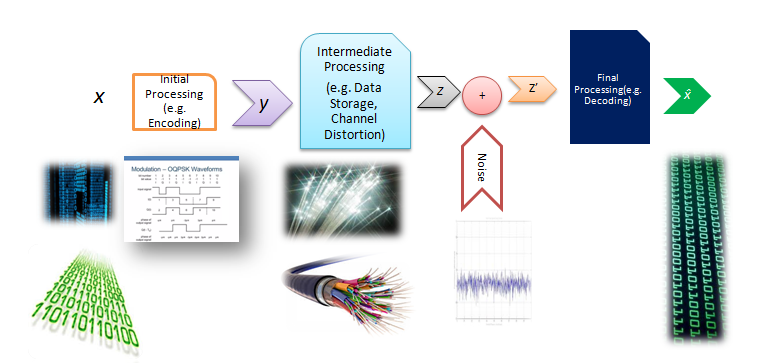
\includegraphics[width=\textwidth]{./Figures/comm_block.png}
  \caption{The general block diagram depicting the processing and recovery of data}
  \label{fig:comm_block}
\end{figure}

Ideally, we want the retrieved data $\hat{x}$ to be equal to the original data $x$ so that the error e defined as $x-\hat{x}$  is $0$; however, this is mostly unachievable due to various factors; noise, interference, hardware nonlinearities such as amplifier saturation. In addition to these external factors that are normally not in our control, there are also limitations inherent in the assumptions and models we employ that may not be adequate in capturing the complexities of the system. Hence, we try to minimize the error through various algorithms and signal processing techniques that have solid mathematical foundations. Nonetheless, these traditional techniques are as good (or bad) in capturing the complexities of our data as our models and assumptions! \\
The use of deep learning can greatly enhance error optimization. The Neural Network learns the model on its own by fitting the training data –labeled or unlabeled- into the model to minimize a particular loss function; this eliminates the inefficiencies that were concomitant with the modeling the system. By iterating through the batches of training data for a sufficient number of epochs, the neural network finds the optimal sets of weights that result in minimal loss. We can view the neural network as the model in itself! But, care must be taken in generalizing this statement; the caveat here is that nonlinear models can only be learned using neural networks with nonlinear activation functions!\\
In communication systems, when the (modulated) data is transmitted through a channel (Copper Wires, Optical Fibers, Air, Water e.t.c ), it is convolved with the channel’s impulse response and corrupted by noise and disturbances. Data at the receiver is vastly different than the one that was originally transmitted. Hence, the receiver is encumbered with the additional task of deconvolving and the denoising the received data. If it were not for the noise and channel impulse response, the received data could have been demodulated to $100\%$ accuracy ($0$ BER) by merely reversing the explicit processes that take place at the modulator and the transmitter. The block diagram for an OFDM system Figure \ref{fig:trad_ofdm} is given below: \\
\begin{figure}[htbp]
  \centering
  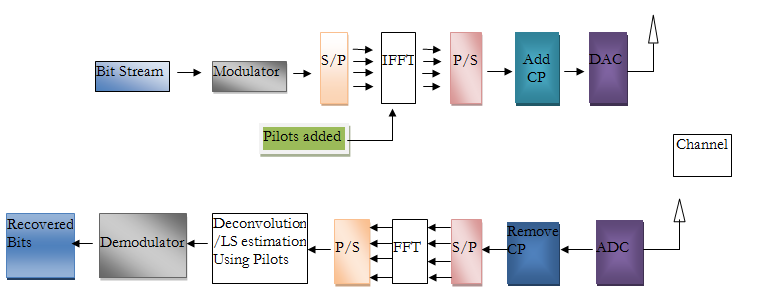
\includegraphics[width=\textwidth]{./Figures/trad_ofdm.png}
  \caption{A traditional single-user OFDM system}
  \label{fig:trad_ofdm}
\end{figure}
The effects of noise and channel distortion are highly nonlinear. This is why the use of linear operations to deconvolve and de-noise the received signal only yields limited success. The ability of the neural network to learn the nonlinear features of a system can be used to great advantage. Nonlinear activation functions like ReLU, Sigmoid, Tanh enable the network to learn complex features that would otherwise be overlooked by traditional methods. In the case of OFDM, we can transmit known data bits through the channel, save the corresponding received signals, and train the neural network using this determinate data.
\begin{figure}[htbp]
  \centering
  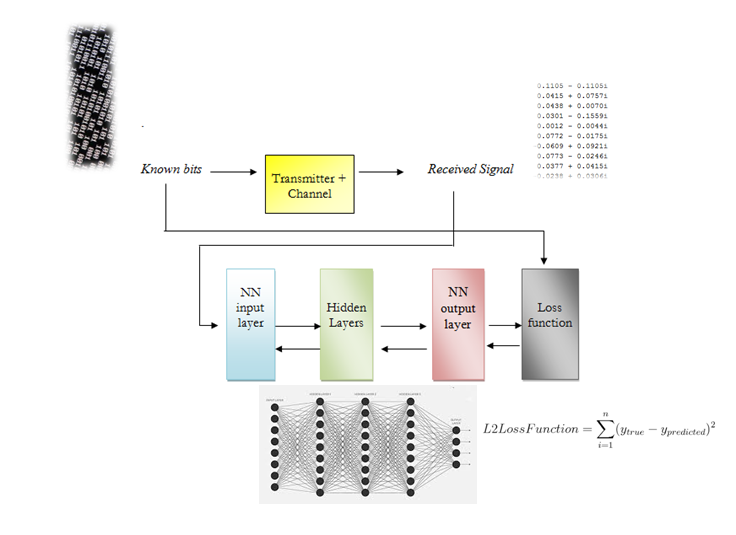
\includegraphics[width=\textwidth]{./Figures/comm_dnn.png}
  \caption{The Receiver is replaced by a Dense Neural Network (DNN)}
  \label{fig:comm_dnn}
\end{figure}
To minimize the loss function, the neural networks updates its weights using optimizers such as Stochastic Gradient Descent (SGD) and Adam’s optimizer, and in the process, learns these two things about the system:
\begin{enumerate}
\item The processes that take place on the transmitter side (e.g., Modulation, CP addition, Pilots, etc.).
\item The features of the channel and the noise that distort the transmitted data
\end{enumerate}
Once the loss has been minimized to a sufficient degree, we use the trained neural network to replace the entire receiver side except DAC. This is illustrated in Figure \ref{fig:comm_dnn} and Figure \ref{fig:comm_comparison}.\\
We also extend the block diagram above for multi-user detection, in which a single receiver recovers the data bits transmitted from 2 independent users using the Non-Orthogonal Multiple Access (NOMA) scheme. 
\begin{figure}[htbp]
  \centering
  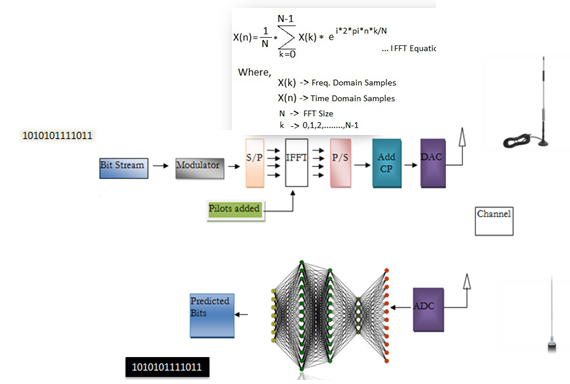
\includegraphics[width=\textwidth]{./Figures/comm_comparison.png}
  \caption{A complete OFDM system with a DNN as its receiver}
  \label{fig:comm_comparison}
\end{figure}
\subsection{Application in Bioinformatics}
For medical applications, we are working towards early diagnosis of Parkinson’s disease (PD). It affects more than 6 million people worldwide and is the second most common neurodegenerative disease after Alzheimer’s disease. There are a myriad number of symptoms for Parkinson's and these symptoms of PD progressively worsen over time, leading to a stark loss in quality of life, and a significant reduction in life expectancy. A detailed account of the Parkinson's symptoms is shown in Figure \ref{fig:park_symp}.
\begin{figure}[htbp]
  \centering
  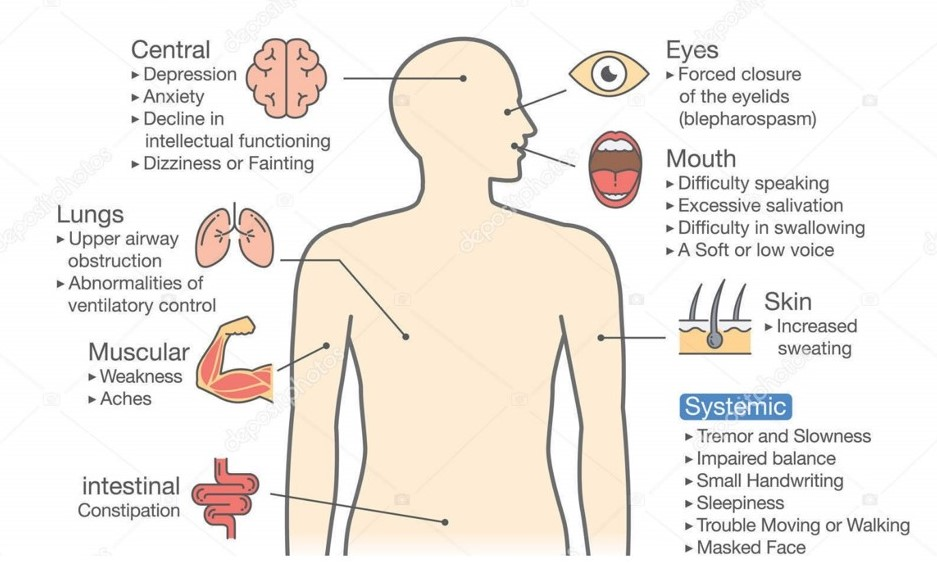
\includegraphics[width=\textwidth]{./Figures/park_symp.jpg}
  \caption{An Illustration of Parkinson's Symptoms}
  \label{fig:park_symp}
\end{figure}
Receiving a timely and accurate diagnosis is paramount for patients because access to treatments could improve their quality of life \cite{global2002factors}. So far, the traditional methods of diagnosing PD are based on subjective clinical assessments of patient’s symptoms. However, research has shown that around 25\% of this diagnosis are incorrect when compared to the results of post-mortem autopsy \cite{pahwa2010early}. These diagnoses are difficult because there are other diseases that may appear similar to PD and symptom severity may fluctuate over time \cite{pahwa2010early}. Adding to that, patients In this project, we explore the possibility of using smartPhone data collected by SageBionetworks, and made public under the umbrella of mPower study, to diagnose people with PD \cite{bot2016mpower}. Such an approach frees the diagnosis process from sporadic clinical trials and gives one the ability to do it anytime one wants. Also, this lets us explore the possibility of using deep-learning models for diagnosis task, which may improve significantly on the previous results.
\begin{figure}[htbp]
  \centering
  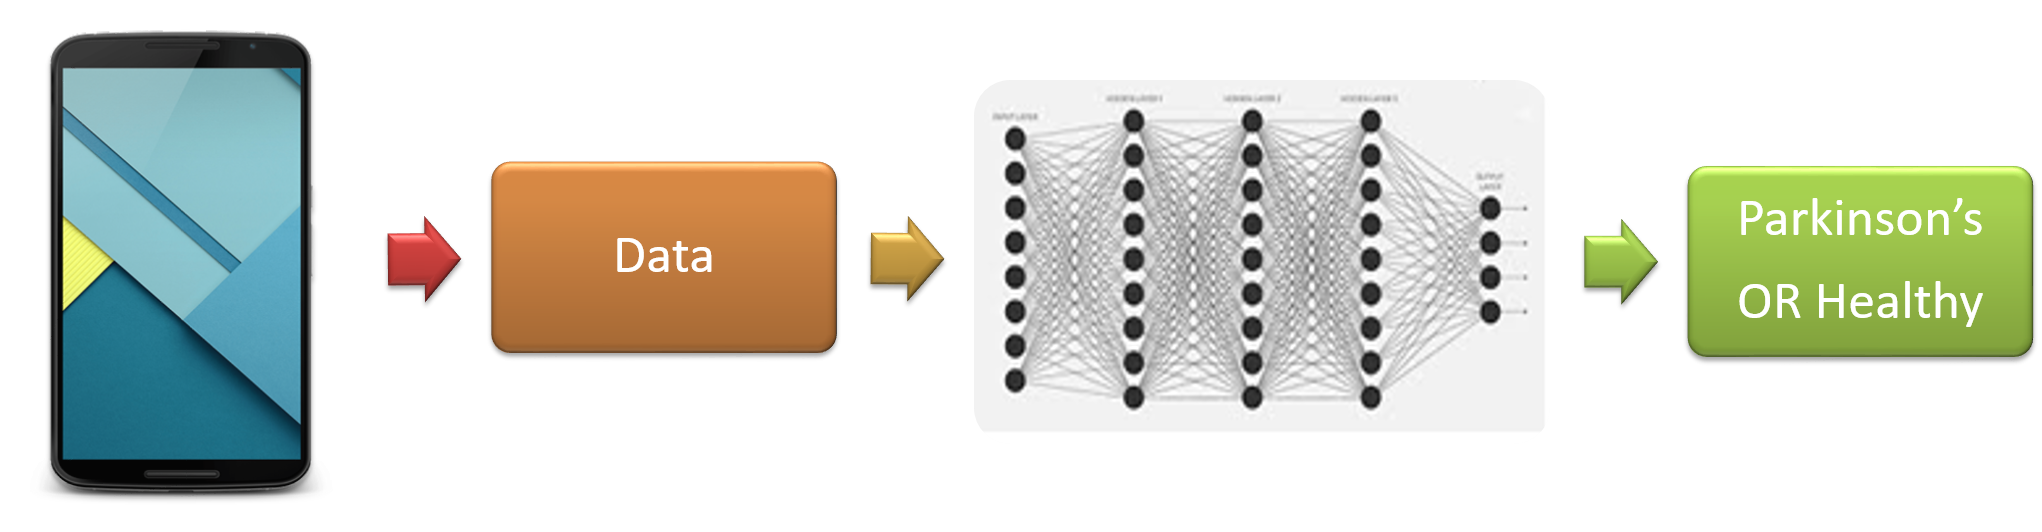
\includegraphics[width=\textwidth]{./Figures/park_dnn.png}
  \caption{A General Block Diagram for the Parkinson's Diagnosis}
  \label{fig:park_dnn}
\end{figure}

The model that we propose for the detection for the early diagnosis of Parkinson's is to optimize a Deep Learning Model that takes in data from Smartphone (Here we use the data already collected under the mPower study) and makes predictions based on this data input as shown in Figure \ref{fig:park_dnn}.
\section{Social Benefits And Relevance}
Information processing systems and health are at the heart of today’s globalized world. Our project targets two very important areas of social significance. If we are able to achieve better performance in these applications, we will impact a great number of people who use these technologies in their everyday lives.

Specifically, the application in Bioinformatics has great potential to affect people's quality of life. The traditional method for Parkinson's diagnosis is clinical diagnosis which is cumbersome and even then misclassifies 25\% of Parkinson's cases \cite{pahwa2010early}. Also, given that Parkinson's shares many of the symptoms with other diseases, patients usually are not motivated to go for a full-fledged clinical diagnosis process, which may lead to worsening of Parkinson's until the point of no recovery. However, if we are able to achieve a good enough performance on our project, we may be able to provide a rough heuristic (if not a complete diagnosis) for people to get themselves professionally checked for PD and that kind of early diagnosis can dramatically improve people's quality of life \cite{pahwa2010early}. 
\section{Goals}
Since this was primarily a research project, our goals were intended to evolve with time as we were to complete our initial deliverables and sift through a sufficient amount of research papers and other resource materials. For communication systems, our primary goal was to first minimize the Bit Error Rate (BER) for complex channel models in simulation for different communication systems (e.g., OFDM, NOMA), and compare them with the traditional methods of equalization; this was somewhat achieved. 

With regards to application in bioinformatics, we targeted the early and easy access self-monitoring of PD using smartphones. We aimed to build towards developing deep learning models which could be deployed on smartphones and can efficiently predict if people have PD using smartphones. Specific activities designed to trigger Parkinson's symptoms were to be performed and recorded on smartphones, which were then to be input to our Deep Learning model giving us the predictions.
\section{Objectives}
Our objective was to achieve the performance of the Neural Network that would be on par with the traditional methods. Once that was attained, we added complexities to our system so that the implementation of the network would become more accurate and more practical.  
\section{Outcomes}
The areas we are working on have a big part to play in the modern world. If we are able to improve on the performance of these algorithms, it will have direct implications on the Information Processing tasks and the Health of people all around the world. This could potentially mean a better world for all of us.
\section{Deliverables (Outputs)}
\textit{As our main motive is to improve on the hand-crafted algorithms in Information Processing and health, for both of our investigations: one into modulation and demodulation blocks of communication systems and the other into diagnosis of PD using smart phone data, we intend to deliver functional and trained deep neural networks which are able to perform the tasks mentioned. We also intend to compare the performance of our frameworks with current hand-crafted algorithms.}
\section{Timelines and the distribution of work}
\begin{figure}[htbp]
  \centering
  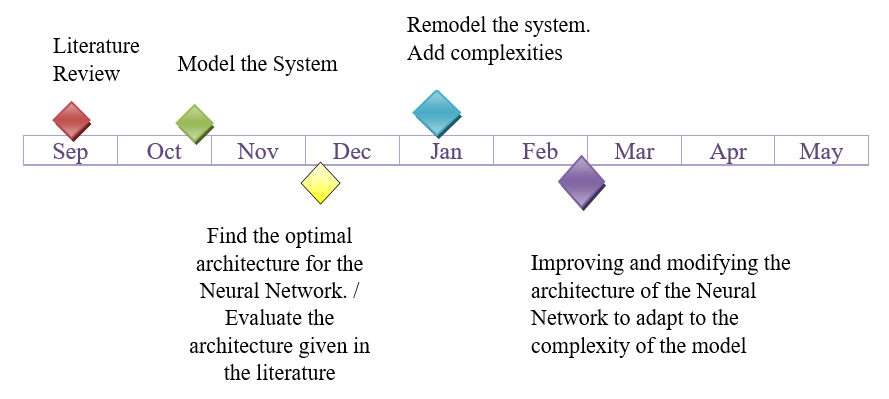
\includegraphics[width=\textwidth]{./Figures/timeline.png}
  \caption{The general summary of the timeline of our work}
  \label{fig:timeline}
\end{figure}
For application in communication systems, we had modeled the OFDM system by the end of September. It took us merely a week to verify the results of the paper our work depended on which consisted of training a Dense Neural Network with the specified architecture. The only deviation from the paper was that we did not use WINNER II and instead used Real Gaussian Channel unchanging across frames. In November, we made the channel complex and increased the number of channel variations, and recorded results for different SNRs. Until December, we worked on Single User Detection. However, in January, we decided to extend our work to the multi-user system and used NOMA. By February, we had tried different architecture for the increased complexity of the system. We found out that the architecture that gave us the best results was a mere extension of the DNN we used for single user detection. We added more neurons to our networks and added a dropout layer to prevent overfitting. In March and April, we compared the performance of our Neural Network against the benchmarks set by the traditional methods. 

For application in bioinformatics, we had reviewed the literature and gained access to the mPower study data. By the End of October, we were successful in restructuring the data to input it into our model. By December, we had successfully implemented the spline CNN \cite{balestriero2018spline} for the classification of Parkinsons's voice data recordings. Later, in January, we implemented a policy for the reclassification of data according to a fixed number of recordings per person. After this policy implementation, we moved on to the implementation of an Evidence Aggregation Model to finally output the predictions for each person. In March and April, we compared the performance of our Neural Network architecture against the benchmarks set by the traditional methods.
